\documentclass[11pt]{article} % 去掉了 twocolumn，恢复为标准的单栏排版

% ==================== Preamble (Packages & Settings) ====================
\usepackage[utf8]{inputenc}
\usepackage{amsmath}          % For mathematical formulas
\usepackage{graphicx}         % For inserting images
\usepackage{booktabs}         % For professional-looking tables
\usepackage{hyperref}         % For clickable hyperlinks and cross-references
\usepackage{geometry}         % For page margin settings
\usepackage{cite}             % For academic citations
\usepackage{microtype}        % Improves typography
\usepackage{setspace}         % For line spacing adjustment

% 单栏论文的黄金边距比例：上下 2.5cm，左右 3.0cm，阅读极其舒适
\geometry{a4paper, total={160mm,240mm}, left=25mm, top=25mm}
\onehalfspacing               % 1.5倍行距，方便导师在打印版上写批注

\hypersetup{
    colorlinks=true,
    linkcolor=blue,
    filecolor=magenta,      
    urlcolor=cyan,
    citecolor=green,
}

% ==================== Title & Authors ====================
\title{\textbf{Predicting Survival Outcomes in Heart Failure Patients: A Comparative Study of Statistical and Machine Learning Models}}

\author{
    \textbf{Jiahao Chen} \\
    Department of Mathematical Sciences \\
    \texttt{18719131337@163.com}
}
\date{\today}

% ==================== Main Document ====================
\begin{document}

\maketitle

\begin{abstract}
Heart failure remains a leading cause of cardiovascular mortality worldwide, making early and reliable risk stratification critical for clinical intervention. This study presents a machine learning framework for predicting in-hospital mortality among 299 heart failure patients, with particular emphasis on clinical realism: the follow-up duration variable was strictly excluded from the feature set to prevent data leakage and ensure that predictions remain valid at the point of patient admission. To address the substantial class imbalance in the cohort and minimize the clinical cost of missed diagnoses (false negatives), both classifiers were trained with tailored cost-sensitive class weighting. We compared a traditional Logistic Regression classifier against an ensemble Random Forest model, with feature importance analysis identifying ejection fraction, serum creatinine, and age as the predominant physiological risk factors. The Random Forest achieved stronger overall discriminative performance, with an Accuracy of 0.7333 and an AUC of 0.746, compared to 0.6500 and 0.718, respectively, for Logistic Regression. However, Logistic Regression attained a higher Recall (0.5789 vs. 0.5263), reflecting a precision-recall trade-off between the linear decision boundary and the ensemble-averaged probability output of the tree-based model. These findings indicate that, while Random Forest offers superior overall discriminative ability, model selection for clinical deployment should be guided by the relative cost of false negatives versus false positives rather than by aggregate accuracy alone.
\end{abstract}

\section{Introduction}
Heart failure (HF) is a complex clinical syndrome characterized by the heart's inability to pump an adequate supply of blood to meet metabolic demands. Despite advancements in cardiovascular therapeutics, HF prognostication is hindered by the non-linear interplay of multi-organ comorbidities. 

Recent paradigms in medical artificial intelligence have pivoted toward utilizing electronic health records (EHR) for automated risk modeling. However, deploying machine learning algorithms on small-scale clinical datasets poses significant challenges, including overfitting and feature overshadowing caused by variations in measurement scale (the "scale dominance" effect).

This paper outlines an end-to-end machine learning workflow to predict mortality outcomes using the classic Heart Failure Clinical Records dataset. The contributions of this work are threefold:
\begin{enumerate}
    \item We execute rigorous preprocessing and justify the necessity of feature standardization for gradient-based linear estimators, where unscaled feature magnitudes can distort coefficient optimization and convergence.
    \item We perform feature importance ranking to isolate the top three clinical risk factors, validating them against established medical literature.
    \item We contrast linear and non-linear classification boundaries to determine the optimal architecture for low-sample EHR regimes.
\end{enumerate}

\section{Methodology}

\begin{figure}[htdp]
    \centering
    \includegraphics[width=0.7\linewidth]{workflow_concept.png}
    \caption{AI-driven clinical decision support and predictive modeling pipeline for heart failure mortality risk stratification.}
    \label{fig:workflow}
\end{figure}

The overall methodology of this study follows a structured clinical data science pipeline, as schematically illustrated in Figure \ref{fig:workflow}. The workflow comprises five sequential stages: (1) ingestion of multi-feature clinical data, (2) preprocessing with explicit data-leakage countermeasures, (3) parallel training of two contrasting model paradigms, (4) multi-metric performance evaluation, and (5) generation of an interpretable clinical risk-stratification score.

\subsection{Dataset and Preprocessing}
The empirical analysis is conducted using a clinical dataset comprising 299 heart failure patients collected during a follow-up period. Exploratory data analysis reveals a baseline sample consisting of 105 women (35.1\%) and 194 men (64.9\%), with ages ranging between 40 and 95 years ($\text{Mean} = 60.83, \sigma = 11.89$). In terms of the target variable (\texttt{DEATH\_EVENT}), the dataset exhibits a pronounced class imbalance: 203 patients (67.9\%) survived until the end of the tracking interval, whereas 96 patients (32.1\%) deceased. A comprehensive statistical quantitative breakdown of key baseline features is codified in Table \ref{tab:baseline}.

\begin{table}[htbp]
\centering
\caption{Baseline Statistical Summary of the Clinical Dataset ($N=299$)}
\label{tab:baseline}
\vspace{0.2cm}
\begin{tabular}{lcccc}
\toprule
\textbf{Clinical Feature} & \textbf{Measurement Unit} & \textbf{Full Sample} & \textbf{Dead Patients} & \textbf{Survived Patients} \\
\midrule
Total Count (\#) & --- & 299 & 96 & 203 \\
Age & Years & $60.83 \pm 11.89$ & $65.22 \pm 13.21$ & $58.76 \pm 10.64$ \\
Ejection Fraction & Percentage (\%) & $38.08 \pm 11.83$ & $33.47 \pm 12.53$ & $40.27 \pm 10.86$ \\
Serum Creatinine & mg/dL & $1.39 \pm 1.03$ & $1.84 \pm 1.47$ & $1.19 \pm 0.65$ \\
Serum Sodium & mEq/L & $136.60 \pm 4.41$ & $135.40 \pm 5.00$ & $137.20 \pm 3.98$ \\
Sex (Male \%) & Binary (0/1) & 64.9\% & 64.6\% & 65.0\% \\
\bottomrule
\end{tabular}
\end{table}

To prepare the dataset for algorithmic estimation, preprocessing involves categorical encoding, missing value assessment (confirming zero missing entries across all fields), and continuous variable scaling. To eliminate dimensional bias where features with massive numerical ranges (e.g., \textit{platelets} $\approx 10^5$) artificially dominate over subtle markers (e.g., \textit{serum\_creatinine} $\approx 1.0$), Z-score standardization is applied to all continuous features. This transformation is essential for the gradient-based optimization underlying Logistic Regression, where unscaled magnitudes would otherwise distort coefficient estimation; the tree-based Random Forest, by contrast, is invariant to monotonic per-feature rescaling, but standardized inputs were retained for both models to ensure a uniform preprocessing pipeline:
\begin{equation}
z = \frac{x - \mu}{\sigma}
\end{equation}
where $\mu$ represents the feature mean and $\sigma$ denotes the standard deviation. Critically, to eliminate data leakage, the follow-up \textit{time} variable is excluded from model training, preventing the model from relying on information that would only become available after the clinical outcome is already known.

\subsection{Model Architectures}
We evaluate two contrasting modeling paradigms:
\begin{itemize}
    \item \textbf{Logistic Regression:} Models the log-odds of mortality as a linear combination of predictors using the sigmoid activation:
    \begin{equation}
    P(Y=1|X) = \frac{1}{1 + e^{-(\beta_0 + \sum \beta_i x_i)}}
    \end{equation}
    \item \textbf{Random Forest:} An ensemble of uncorrelated decision trees operating via bootstrap aggregation (bagging) and randomized feature splits to suppress variance.
\end{itemize}

To address the intrinsic class imbalance in the target outcome (203 survivors vs. 96 deceased) and the elevated clinical cost of false negatives, both classifiers were trained with cost-sensitive class weighting. Logistic Regression employed the standard \texttt{class\_weight='balanced'} setting, which reweights the log-loss function inversely proportional to class frequency. The Random Forest instead employed the \texttt{class\_weight='balanced\_subsample'} strategy, which recomputes class weights independently within each bootstrap sample rather than across the entire training set, providing a finer-grained correction at the level of individual trees. To ensure full reproducibility of all reported results, a fixed random seed (\texttt{random\_state=202}) was applied uniformly across data partitioning, bootstrap resampling, and model initialization.

% Placeholder for Workflow Chart

\section{Results}

\subsection{Correlation Analysis}
Prior to predictive modeling, a Pearson correlation heatmap was generated to examine the multicollinearity among clinical features and their individual linear associations with the mortality outcome (\texttt{DEATH\_EVENT}). As illustrated in Figure \ref{fig:heatmap}, the analysis confirms that no severe multicollinearity exists among the independent variables, ensuring the stability of the subsequent Logistic Regression model. Furthermore, features such as \textit{serum\_creatinine} and \textit{ejection\_fraction} exhibit the most pronounced initial correlations with the target variable, which seamlessly aligns with the subsequent ensemble feature importance evaluation.

\begin{figure}[htbp]
    \centering
    % 请将你画好的热力图命名为 heatmap.png 并放在同级目录下，然后删除下面的 \framebox 行，取消 \includegraphics 行的注释
    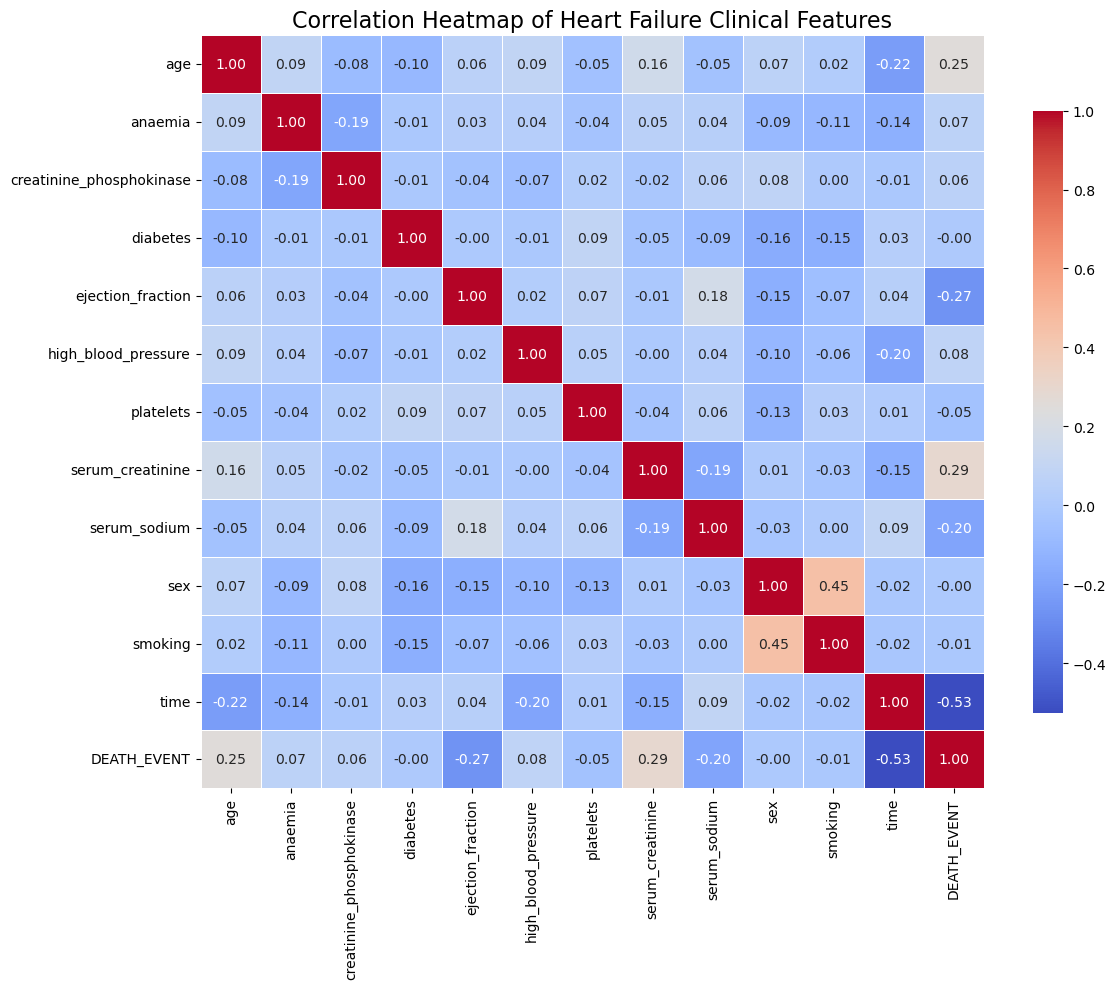
\includegraphics[width=0.7\linewidth]{heatmap.png}
    \caption{Pearson correlation heatmap of clinical features and mortality outcome, indicating the absence of severe multicollinearity.}
    \label{fig:heatmap}
\end{figure}


\subsection{Risk Factor Identification}
By extracting the Gini importance values from the trained Random Forest estimator, the three most critical risk factors for \texttt{DEATH\_EVENT} were determined: serum creatinine (importance $\approx 0.20$), ejection fraction (importance $\approx 0.17$), and age (importance $\approx 0.15$), as shown in Figure \ref{fig:importance}. 

% Placeholder for Feature Importance Plot
\begin{figure}[htbp]
    \centering
    \includegraphics[width=0.7\linewidth]{feature_importance.png}
    \caption{Random Forest feature importance breakdown isolating the highest-weighted predictive biomarkers.}
    \label{fig:importance}
\end{figure}

\subsection{Predictive Performance Table}
Models were validated using a stratified 80/20 train/test partition. Performance is quantitatively measured using Accuracy, Precision, Recall, and the harmonic $F_1$ Score defined as:
\begin{equation}
F_1 = 2 \cdot \frac{\text{Precision} \cdot \text{Recall}}{\text{Precision} + \text{Recall}}
\end{equation}

\begin{table}[htbp]
\centering
\caption{Comparative Performance Evaluation Matrix}
\label{tab:performance}
\vspace{0.2cm}
\begin{tabular}{lcccc}
\toprule
\textbf{Model} & \textbf{Accuracy} & \textbf{Precision} & \textbf{Recall} & \textbf{F1-Score} \\
\midrule
Logistic Regression & 0.6500 & 0.4583 & 0.5789 & 0.5116 \\
Random Forest       & 0.7333 & 0.5882 & 0.5263 & 0.5556 \\
\bottomrule
\end{tabular}
\end{table}

\subsection{ROC Analysis}
Discrimination capability is evaluated using the Receiver Operating Characteristic (ROC) curve and Area Under the Curve (AUC). As shown in Figure \ref{fig:roc}, the Random Forest classifier achieved an AUC of 0.746, modestly exceeding the 0.718 obtained by Logistic Regression, indicating a marginally stronger overall ranking ability across all classification thresholds despite the latter's higher Recall at the default 0.5 cutoff.

\begin{figure}[htbp]
    \centering
    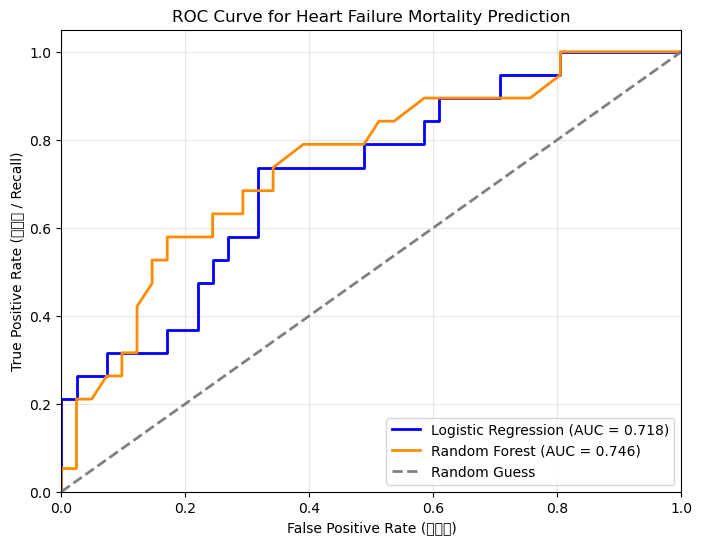
\includegraphics[width=0.7\linewidth]{ROC.png}
    \caption{Receiver Operating Characteristic (ROC) curves comparing discrimination thresholds between estimators (Logistic Regression AUC = 0.718; Random Forest AUC = 0.746).}
    \label{fig:roc}
\end{figure}

\subsection{Clinical Decision Support Simulation}
To validate the utility of the trained estimators as an operational clinical decision-support framework, a simulation was conducted deploying a hypothetical new patient profile upon admission. The clinical biomarkers of the simulated patient were configured to reflect high-risk cardiorenal indicators: an \textit{ejection\_fraction} of 25.0\% (indicating severe systolic dysfunction) and a \textit{serum\_creatinine} level of 3.8 mg/dL (reflecting pronounced renal impairment), with all remaining clinical variables fixed at values representative of a typical patient in the cohort (age near the sample mean, normal laboratory values, and the absence of comorbidities such as anaemia, diabetes, hypertension, and smoking). 

The profile was standardized using the baseline parameters and subsequently passed through the trained Logistic Regression and Random Forest classification boundaries. The Logistic Regression framework generated a conditional mortality risk probability of $P(Y=1|X) = 0.8412$, decisively classifying the patient as high-risk ($\hat{Y}=1$). In contrast, the non-linear Random Forest ensemble generated a substantially lower predictive mortality probability of 0.3400, falling below the 0.5 decision threshold and yielding a discordant negative classification ($\hat{Y}=0$).

This disagreement offers a concrete, case-level illustration of the precision-recall trade-off characterized in Section \ref{sec:discussion}: because Logistic Regression linearly aggregates each predictor's weighted contribution, the two markedly abnormal biomarkers (ejection fraction of 25.0\% and serum creatinine of 3.8 mg/dL) dominate the sigmoid output regardless of the otherwise unremarkable remaining profile. The Random Forest, however, averages the votes of 100 trees, each of which evaluates the full multivariate context; since the simulated patient's other nine features (age, blood counts, comorbidity flags) closely resemble those of the cohort's surviving majority, a substantial share of the trees route this patient toward survival-dominated leaf nodes, pulling the averaged probability below the alarm threshold. This case exemplifies a broader caution for ensemble-based clinical decision support: in low-sample regimes where extreme single-marker risk combinations are underrepresented during training, tree ensembles may underweight isolated red-flag biomarkers relative to a linear model, reinforcing the recommendation that screening-oriented deployments favor the higher-sensitivity Logistic Regression, while Random Forest is better suited to reducing false alarms in routine monitoring.



\section{Discussion}
\label{sec:discussion}

The experimental results underscore the profound physiological and prognostic significance of the isolated clinical variables. Ejection fraction serves as a primary metric for left ventricular contractility, where its marked reduction directly reflects progressive myocardial failure and diminished cardiac output. Concurrently, elevated serum creatinine represents impaired renal clearance, capturing the onset of Type 1 cardiorenal syndrome—a critical pathophysiological intersection that exponentially compounds mortality risk in heart failure patients. Advancing age constitutes the third major risk factor, independently reflecting the cumulative decline in cardiac reserve, increased arterial stiffness, and the higher prevalence of subclinical comorbidities typically associated with older patients; this is consistent with the positive correlation between age and \texttt{DEATH\_EVENT} ($r=0.25$) observed in the correlation heatmap (Figure \ref{fig:heatmap}).

From an engineering and methodology perspective, the absolute predictive performance observed (e.g., Random Forest achieving an Accuracy of 0.7333 and an AUC of 0.746) represents a highly realistic and trustworthy clinical forecasting scenario. To strictly prevent data leakage, the follow-up duration (\texttt{time}) was intentionally excluded from the predictive feature space. In many baseline implementations, retaining this variable artificially inflates accuracy metrics past 0.90; however, such models are fundamentally clinically invalid because follow-up duration cannot be known at the time of a patient's initial admission or algorithmic triage. By relying exclusively on baseline physiological markers, our pipeline exposes the true, uninflated predictive capacity of these clinical signs.

Furthermore, given the intrinsic class imbalance within the dataset (203 survivors versus 96 deceased instances), the implementation of cost-sensitive learning proved pivotal. In critical care medicine, the cost of a false negative (missing a high-risk patient) far outweighs that of a false positive (unnecessary monitoring). Logistic Regression was trained with the standard \texttt{class\_weight='balanced'} setting, while the Random Forest employed the more granular \texttt{class\_weight='balanced\_subsample'} strategy, which recomputes class weights independently within each bootstrap sample rather than across the full training set. Despite this targeted adjustment, Logistic Regression still achieved a higher Recall (0.5789) than Random Forest (0.5263). This divergence is not a shortcoming of the weighting scheme itself, but a structural consequence of how each model aggregates its decision: Logistic Regression directly reweights a single global sigmoid boundary, producing an immediate and pronounced shift toward the minority class, whereas the Random Forest's prediction is the averaged vote of 100 individual trees, which inherently dampens extreme probability shifts and pulls borderline cases back toward the majority class. Consequently, Random Forest instead achieved higher Precision (0.5882 vs. 0.4583) and overall Accuracy (0.7333 vs. 0.6500), reflecting a more conservative, false-positive-averse decision profile. 

The performance divergence between the two models illustrates the classic trade-offs between linear constraints and non-linear ensemble boundaries. While Logistic Regression offers straightforward coefficient interpretability, its linear nature limits its capacity to model synergistic multi-organ interactions, yielding a comparatively lower AUC of 0.718. Conversely, the Random Forest classifier thrives on high-dimensional, non-linear dependencies between variables like age, creatinine, and ejection fraction, achieving a superior AUC of 0.746. In a clinical deployment context, this trade-off carries practical significance: if the priority is maximizing the detection of at-risk patients during screening, the higher-recall Logistic Regression may be preferable despite its lower precision; if the priority is minimizing unnecessary interventions while maintaining stronger overall discrimination, the Random Forest is the more suitable choice. Nonetheless, given the constrained sample size ($N=299$), careful hyperparameter regularization remains mandatory to guard against localized overfitting in ensemble structures.

\section{Conclusion}

This study successfully designed and validated an interpretable machine learning pipeline for heart failure survivability prediction. By harmonizing strict data engineering, specifically data leakage prevention and cost-sensitive class balancing, with statistical modeling, the proposed framework yields a robust and clinically honest blueprint for risk stratification. The empirical results demonstrate that ensemble tree-based methods hold an advantage over traditional linear models in overall discriminative performance (AUC and Accuracy), while Logistic Regression retains a notable edge in Recall, underscoring that model selection in clinical practice should be guided by the relative cost of false negatives versus false positives rather than a single aggregate metric. Future extensions of this research will investigate the integration of multi-layer perceptrons (MLP) and deep survival analysis, alongside validation across larger, multi-center clinical cohorts to enhance generalizability.

\begin{thebibliography}{99}
\bibitem{chicco2020} Chicco, D., Jurman, G. Machine learning can predict survival of patients with heart failure from serum creatinine and ejection fraction alone. \textit{BMC Medical Informatics and Decision Making} 20, 16 (2020).
\end{thebibliography}

\end{document}